\documentclass[10pt,dvipsnames, aspectratio=169]{beamer}
\usepackage{graphicx}
\usepackage{caption}
\usepackage{subcaption}
%\newcommand{\source}[1]{\caption{Source:{#1}} }
\author{Md. Jubayer Hossain \\ \url{https://jhossain.me/} \\ jubayer@hdrobd.org}
\title{Introduction to Scientific Computing for Biologists}
\institute{Founder \\ Health Data Research Organization \\ Lead Organizer \\ 
Scientific Computing for Biologists  }
\subtitle{ISCB20.09 -- Interpreting Data Using Descriptive Statistics with R}
\begin{document}
	% Slide-n
	\begin{frame}
		\maketitle
	\end{frame}

% Section-1: Introduction 
	\begin{frame}[t]{Statistics and Biostatistics: Definitions--1}
		\textbf{Definition--1: What is Statistics?} \\
		Statistics is the discipline that concerns the collection, 
		organization, 
		analysis, interpretation and presentation of data. In applying 
		statistics 
		to a scientific, industrial, or social problem, it is conventional to 
		begin 
		with a statistical population or a statistical model to be studied. 
		(Source: \url{https://en.wikipedia.org/wiki/Statistics})
		
		\textbf{Definition--2: What is Statistics?}\\ 
		Simply, Statistics is a branch of mathematics that deals with 
		collecting,
		organizing, analyzing, and interpreting data. 
		(Source: 
		\url{https://app.pluralsight.com/library/courses/interpreting-data-descriptive-statistics-python/})
	\end{frame}

	\begin{frame}[t]{Statistics and Biostatistics: Definitions--2}
		\textbf{Definition--3: What is Biostatistics?} \\
		Biostatistics is the application of statistics to a variety of topics 
		in 
		biology. In this course, we tend to focus on biological topics in the 
		health sciences as we learn about statistics. 
		(Source: \url{https://bolt.mph.ufl.edu/6050-6052/}) \\ 
		
		\vspace{6pt}
		
		\textbf{Definition--4: What is Biostatistics?} \\
		Biostatistics is the application of statistics to problems in the
		biological sciences, health, and medicine.
		(Source: 
		\url{https://ocw.jhsph.edu/index.cfm/go/viewCourse/course/MethodsInBiostatisticsI/})
		
	\end{frame}

	% Slide-Data-1 
	\begin{frame}[t]{What is Data?}
		\begin{itemize}
			\item \textbf{Definition--1:} Data is a collection of facts, such 
			as 
			numbers, 
			images, words, 
			measurements, observations, audios, videos or just descriptions of 
			things.
			\item \textbf{Definition--2:} Data is a tool to reach suitable 
			conclusion. 
		\end{itemize}
		
		\begin{figure} [ht]
			\centering
			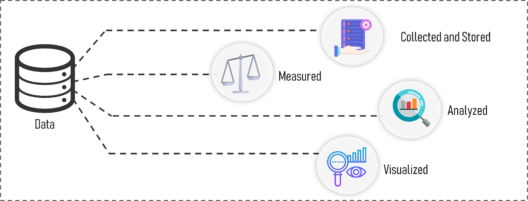
\includegraphics[width=0.8\textwidth]{stats_img/data.png}
			\caption{\url{https://www.edureka.co/blog/statistics-and-probability/}}
		\end{figure}
	\end{frame}
	% Slide-n
	\begin{frame}[t]{Types of Data}
		\begin{figure} [ht] \vspace{20pt}
			\centering
			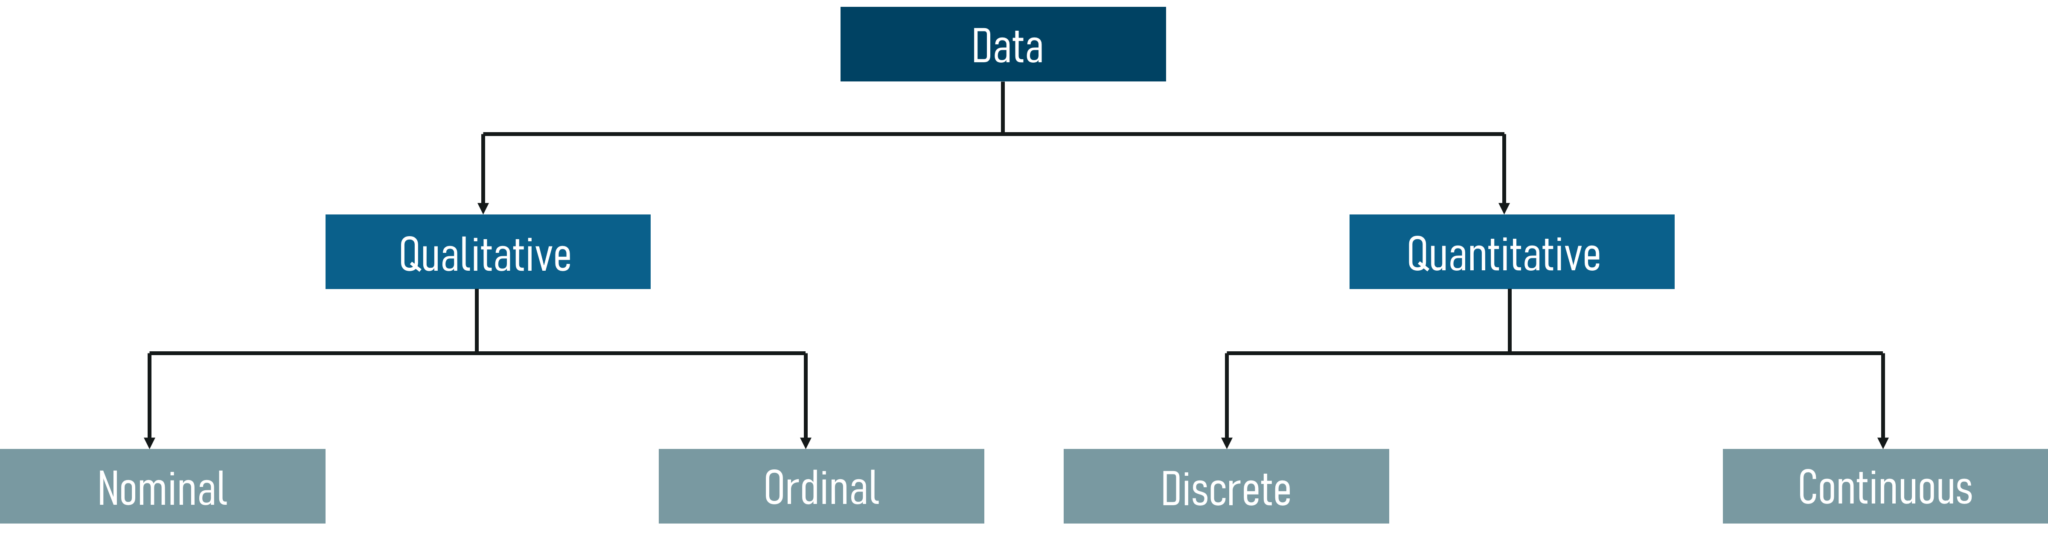
\includegraphics[width=0.98\textwidth]{stats_img/types_of_data.png}
		\end{figure}
	\end{frame}
	
	% Slide-n
	\begin{frame}[t]{Qualitative  or Categorical Data}
		\begin{itemize}
			\item Classifies individuals or items into different groups.
			\item Qualitative data is further divided into two types of data
			\begin{itemize}
				\item[--] \textbf{Ordinal:} groups have an order or ranking.
				\item [--]\textbf{Nominal:} groups are merely names, no ranking.
			\end{itemize}
		\end{itemize}
		
		\begin{figure}[h]
			\centering
			\begin{subfigure}{0.45\textwidth}
				\centering
				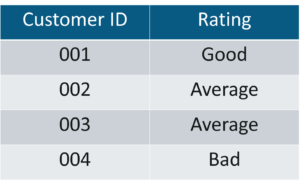
\includegraphics[width=3.5cm, 
				height=3.5cm]{stats_img/ordinal.png}
				\caption{Ordinal Data}
			\end{subfigure}
			\hfil
			\begin{subfigure}{0.45\textwidth}
				\centering
				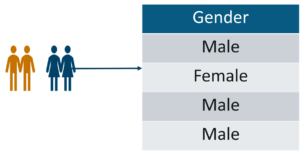
\includegraphics[width=3.5cm, 
				height=3.5cm]{stats_img/nominal.png}
				\caption{Nominal Data}
			\end{subfigure}
			\caption{\url{https://www.edureka.co/blog/statistics-and-probability/}}
		\end{figure}
	\end{frame}


\begin{frame}[t]{Quantitative or Numeric Data}
	\begin{itemize}
		\item Numerical, measurable quantities in which arithmetic
		operations often make sense.
		\item Quantitative data is also further divided into two types of data
		\begin{itemize}
			\item \textbf{Continuous:} could take on any value within an 
			interval,many possible values.
			\begin{itemize}
				\item[--] A person's height: could be any value (within the 
				range 
				of human heights), not just certain fixed heights. 
				\item[--] Time in a race: you could even measure it to 
				fractions of 
				a second.
				\item [--]Blood pressure, mmHg.
				\item [--]Weight, pounds (kilograms, ounces, etc.)
			\end{itemize}
			\item \textbf{Discrete:} countable value, finite number of values.
			\begin{itemize}
				\item[--] The number of students in a class.
				\item[--] The results of rolling a die.
			\end{itemize}
		\end{itemize}
	\end{itemize}
\end{frame}

% Slide-n
\begin{frame}[t]{Binary Data}
	\begin{itemize}
		\item Yes/No
		\item Polio: Yes/No
		\item Cure: Yes/No
		\item Sex: Female/Male(0 or 1)
	\end{itemize}
\end{frame}

\begin{frame}[t]{Types of Variables}
	\begin{itemize}
		\item \textbf{Independent Variable(IV)} \\
		A variable whose value does not change by the effect of other variables 
		and is used to manipulate the dependent variables. It is often denoted 
		as $X$. 
		\item \textbf{Dependent Variable(DV)} 
		A variable whose value change when there is any manipulation in the 
		values of independent variables. Is is often denoted as $Y$
	\end{itemize}
	\centering
	\textbf{$X$ Causes $Y$} \\ 
	$X$ (effect) $\rightarrow$ Year of Experience $\rightarrow$ Independent \\ 
	$Y$ (cause) $\rightarrow$ Salary $\rightarrow$ Dependent
\end{frame}


% Slide-n
\begin{frame}[t]{Other Names for IV and DV}
	\textbf{Other Names for Independent Variables}
	\begin{itemize}
		\item Explanatory Variables (they explain an event or outcome)
		\item Predictor Variables (they can be used to predict the value of a 
		dependent variable)
	\end{itemize} 
	\textbf{Other Names for Dependent Variables}
	\begin{itemize}
		\item Response Variables (they respond to a change in another variable)
		\item Outcome Variables (they represent the outcome you want to measure)
	\end{itemize}
\end{frame}


% Slide-n
\begin{frame}[t]{A Typical Dataset}
	\begin{figure} [ht]
		\centering
		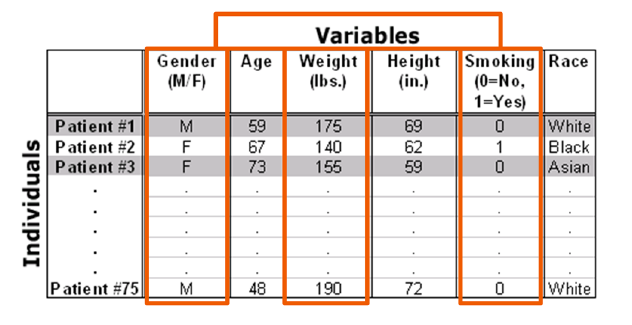
\includegraphics[width=0.5\textwidth]{stats_img/dataset.png}
	\end{figure}
	
	\begin{itemize}
		\item \textbf{Variables} contain the information about a particular 
		characteristic 
		for all individuals in a dataset.
		\item An \textbf{observation} in statistics is a value of something of 
		interest you're measuring or counting during a study or experiment: a 
		person's height, a bank account value at a certain point in time, or 
		number 
		of animals.
	\end{itemize}
	
\end{frame}

\begin{frame}[t]{Terminologies In Statistics: Population and Sample}
	
	\textbf{Population:} The population is the entire group that you want to 
	draw conclusions about.
	
	\textbf{Sample:} The sample is the specific group of individuals that you 
	will collect data from.
	
	\begin{figure} [ht]
		\centering
		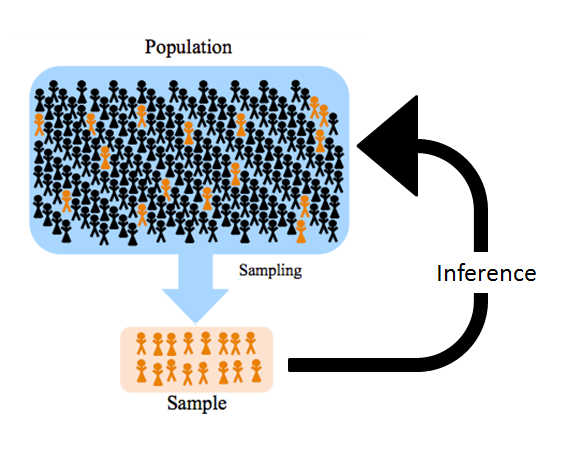
\includegraphics[width=0.5\textwidth]{stats_img/population_sample.png}
		\caption{\url{https://online.stat.psu.edu/stat500/}}
	\end{figure}
\end{frame}


\begin{frame}[t]{Terminologies In Statistics: Sampling Frame and Sample Size}
	
	\textbf{Sampling Frame} \\ 
	The sampling frame is the actual list of 
	individuals that the sample will be drawn from. Ideally, it should include 
	the entire target population (and nobody who is not part of that 
	population).
	
	\textbf{Sample Size} \\ 
	The number of individuals in your sample depends on 
	the size of the population, and on how precisely you want the results to 
	represent the population as a whole.
	
	
	\textbf{Sample Size Calculator} \\
	Surveymonkey--\url{https://www.surveymonkey.com/mp/sample-size-calculator/}
	
\end{frame}


% Slide-n
\begin{frame}[t]{Characteristics of a Good Sample--1}
	\begin{itemize}
		\item \textbf{Goal-oriented:} A sample should be goal oriented. It 
		should be oriented to the research objectives and fitted to the survey 
		conditions. \pause 
		\item \textbf{Acurate representative of the population:} A sample 
		should be an accurate representative of the population from which it is 
		taken. \pause
		\item \textbf{Proportional:} A sample should be proportional. It should 
		be large enough to represent the population properly. In general, the 
		larger the sample size, the more accurately and confidently 
		you can make inferences about the whole population.\pause 
		
		\item \textbf{Random Selection:} A sample should be selected at random. 
		This means that any item in the group has a full and equal chance of 
		being selected and included in the sample.This makes the selected 
		sample truly representative in character. \pause 
		\item \textbf{Economical:} A sample should be economical.The objective 
		of the survey should be achieved with minimum cost and effort. 
		
	\end{itemize}
\end{frame}

\begin{frame}[t]{Characteristics of a Good Sample--2}
	\begin{itemize}
		\item \textbf{Practical:} A sample should be practical. The sample 
		design should be simple. It should be capable of being understood and 
		followed in the fieldwork. \pause 
		\item \textbf{Actual information provider:} A sample should be designed 
		so as to provide actual information required for the study and also 
		provide an adequate basis for the measurement of its own reliability. 
		\pause
	\end{itemize}
\end{frame}


\begin{frame}[t]{Types of Statistics}
	\textbf{There are two kinds of statistics,
		the kind you look up and the kind
		you make up} \\ 
	--Rex Stout
	\begin{itemize}
		\item \textbf{Descriptive Statistics} -- Identify important elements in 
		a
		dataset.
		\item \textbf{Inferential Statistics} -- Explain those elements via
		relationships with other elements.
	\end{itemize}
\end{frame} 

% Slide-n
\begin{frame}[t]{Descriptive Statistics}
	\textbf{Descriptive statistical} methods provide an exploratory assessment 
	of the data from a study. 
	\begin{itemize}
		\item Descriptive statistical methods provide a exploratory data 
		analysis.
		\begin{itemize}
			\item[--] Frequency Distribution Table 
			\item[--] Graphs / Charts 
			\item [--] Summary 
		\end{itemize}
		\item Descriptive statistical methods divide into 3 categories.
		\begin{itemize}
			\item[--] \textbf{Univariate analysis} summarize only one variable 
			at a 
			time.
			\item[--] \textbf{Bivariate analysis}  compare two variables.
			\item [--]\textbf{Multivariate analysis} compare more than two 
			variables.
		\end{itemize}
	\end{itemize}
\end{frame}

% Slide-n
\begin{frame}[t]{Inferential Statistics}
	\textbf{Assess the strength of evidence} for/against a hypothesis; evaluate 
	the data
	\begin{itemize}
		\item Inferential statistical methods provide a confirmatory data 
		analysis
		\begin{itemize}
			\item [--]Generalize conclusions from data from part of a group 
			(sample) to the whole group
			(population)
			\item[--] Assess the strength of the evidence
			\item [--]Make comparisons
			\item [--]Make predictions
		\end{itemize}
		\item Inferential statistical methods divide into 2 categories.
		\begin{itemize}
			\item[--] \textbf{ Hypothesis Testing:} Hypothesis testing is a 
			formal 
			procedure for investigating our ideas about the world using 
			statistics. 
			It is most often used by scientists to test specific predictions, 
			called hypotheses, that arise from theories.
			\item[--] \textbf{Model Fitting:} Model fitting is a measure of how 
			well a statistical learning model generalizes to similar data to 
			that 
			on which it was trained. A model that is well-fitted produces more 
			accurate outcomes.
		\end{itemize}
	\end{itemize}
\end{frame}
% End of Introduction 

% Slide-n
\begin{frame}[t]{Sampling}
	\begin{figure} [ht]
		\centering
		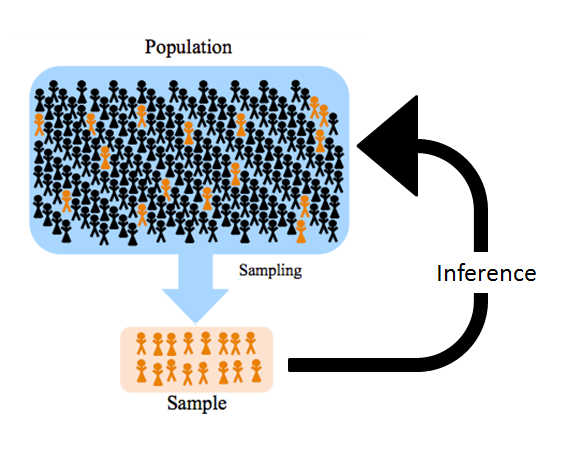
\includegraphics[width=0.6\textwidth]{stats_img/population_sample.png}
		\caption{\url{https://online.stat.psu.edu/stat500/}}
	\end{figure}
\end{frame}

% Slide-n
\begin{frame}[t]{Types of Sampling Methods}
	To draw valid conclusions from your results, you have to carefully decide 
	how you will select a sample that is representative of the group as a 
	whole. There are two types of sampling methods
	\begin{itemize}
		\item Probability Sampling
		\item Non-Probability Sampling 
	\end{itemize}
\end{frame}

% Slide-n
\begin{frame}[t]{Probability Sampling Methods}
	\begin{itemize}
		\item Probability sampling involves 
		random selection, allowing you to make statistical inferences about the 
		whole group.
		\item Probability sampling means that every member of the population 
		has a chance of being selected.
		\item It is mainly used in quantitative research.
		\item If you want to produce results that are representative of the 
		whole population, you need to use a probability sampling technique.
	\end{itemize}
\end{frame}

% Slide-n
\begin{frame}[t]{Non-Probability Sampling Methods}
	\begin{itemize}
		\item Non-probability sampling involves 
		non-random selection based on convenience or other criteria, allowing 
		you to easily collect initial data.
	\end{itemize}
\end{frame}

% Slide-n
\begin{frame}[t]{Types of Probability Sampling Methods}
	\begin{figure} [ht]
		\centering
		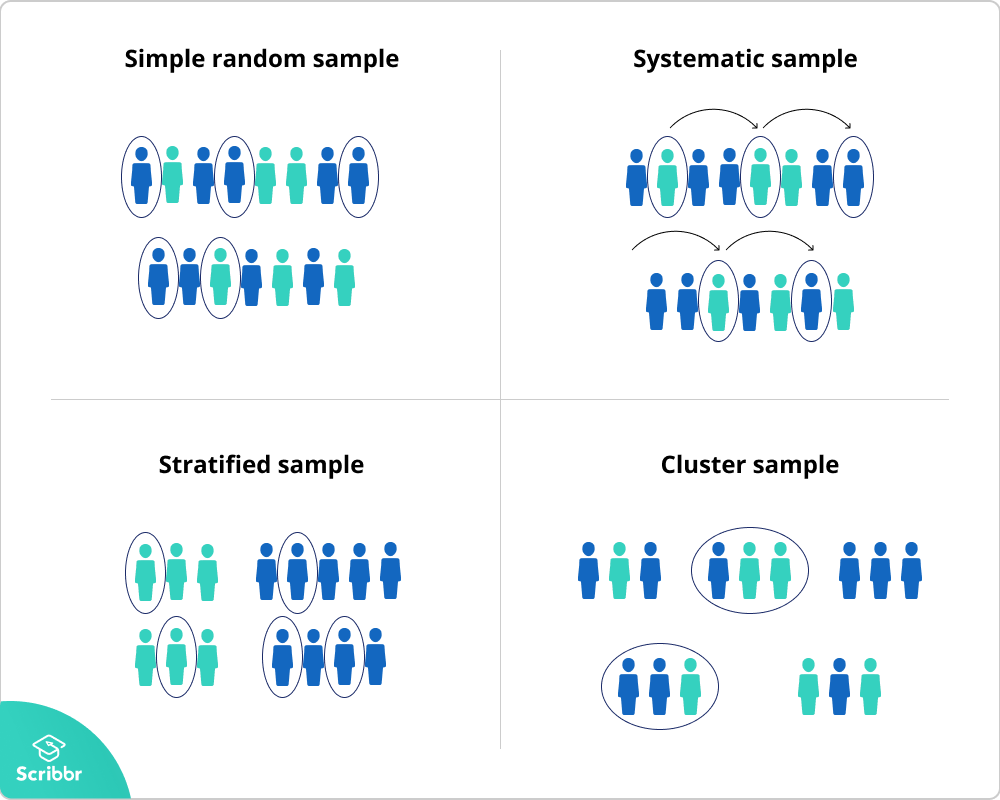
\includegraphics[width=0.6\textwidth]{rp/sampling.png}
		\caption{\url{https://www.scribbr.com/methodology/sampling-methods/}}
	\end{figure}
\end{frame}


% Slide-n
\begin{frame}[t]{Simple Random Sampling(SRS)}
	\begin{itemize}
		\item In a simple random sample, every member of the population has an 
		equal chance of being selected. Your sampling frame should include the 
		whole population.
		\item To conduct this type of sampling, you can use tools like random 
		number generators or other techniques that are based entirely on chance.
	\end{itemize}
\end{frame}
% Slide-n
\begin{frame}[t]{Systematic Sampling}
	\begin{itemize}
		\item Systematic sampling is similar to simple random sampling, but it 
		is usually slightly easier to conduct.
		\item Every member of the population is listed with a number, but 
		instead of randomly generating numbers, individuals are chosen at 
		regular intervals.
	\end{itemize}
\end{frame}

% Slide-n
\begin{frame}[t]{ Stratified Sampling}
	\begin{itemize}
		\item Stratified sampling involves dividing the population into 
		subpopulations that may differ in important ways. It allows you draw 
		more precise conclusions by ensuring that every subgroup is properly 
		represented in the sample.
		\item To use this sampling method, you divide the population into 
		subgroups (called strata) based on the relevant characteristic (e.g. 
		gender, age range, income bracket, job role).
		\item Based on the overall proportions of the population, you calculate 
		how many people should be sampled from each subgroup. Then you use 
		random or systematic sampling to select a sample from each subgroup.
	\end{itemize}
\end{frame}

% Slide-n
\begin{frame}[t]{Cluster Sampling}
	\begin{itemize}
		\item Cluster sampling also involves dividing the population into 
		subgroups, but each subgroup should have similar characteristics to the 
		whole sample. Instead of sampling individuals from each subgroup, you 
		randomly select entire subgroups.
		\item If it is practically possible, you might include every individual 
		from each sampled cluster. If the clusters themselves are large, you 
		can also sample individuals from within each cluster using one of the 
		techniques above.
		\item This method is good for dealing with large and dispersed 
		populations, but there is more risk of error in the sample, as there 
		could be substantial differences between clusters. It’s difficult to 
		guarantee that the sampled clusters are really representative of the 
		whole population.
	\end{itemize}
\end{frame}

% Slide-n
\begin{frame}[t]{Types of Statistical Methods}
	\begin{itemize}
		\item \textbf{Descriptive Statistics:} Identify important elements in a
		dataset.
		\item \textbf{Inferential Statistics:} Explain those elements via
		relationships with other elements.
	\end{itemize}
\end{frame}

% Slide-n
\begin{frame}[t]{Descriptive Statistics}
	Descriptive Statistics divide into 3 categories.
	\begin{itemize}
		\item \textbf{Univariate Analysis:}  summarize only one variable at a 
		time.
		\item \textbf{Bivariate Analysis:}  compare two variables.
		\item \textbf{Multivariate Analysis:}  compare more than two variables.
	\end{itemize}
\end{frame}

% Slide-n
\begin{frame}[t]{Characteristics of Descriptive Statistical Methods}
	\begin{itemize}
		\item Descriptive statistical methods provide an exploratory
		assessment of the data from a study
		\item Exploratory data analysis techniques
		\item Organization and summarization of data
		\begin{itemize}
			\item Tables
			\item Graphs
			\item Summary measures
		\end{itemize}
	\end{itemize}
\end{frame}


\begin{frame}[t]{Inferential Statistics}
	Inferential Statistics divide into 2 categories.
	\begin{itemize}
		\item \textbf{Hypothesis
			Testing:} A hypothesis is a statement that can be tested by 
		scientific research.
		\item \textbf{Model Fitting:} Model fitting is a measure of how well a 
		statistical learning model generalizes to similar data to that on which 
		it was trained.
	\end{itemize}
\end{frame}


% Slide-n
\begin{frame}[t]{Characteristics of Inferential Statistical Methods}
	\begin{itemize}
		\item Assess the strength of evidence for/against a hypothesis.
		\item Inferential statistical methods provide a confirmatory
		data analysis.
		\item Generalize conclusions from data from part of a
		group (sample) to the whole group (population)
		\item Assess the strength of the evidence
		\item Make comparisons.
		\item Make predictions.
		\item Ask more questions; suggest future research.
	\end{itemize}
\end{frame}







\begin{frame}[t]{A Quick Review of Data and Variables--1}
	\begin{itemize}
		\item \textbf{Variable}
		\begin{itemize}
			\item[--]  A characteristic taking on different values. 
		\end{itemize}
	\end{itemize}
	
	\begin{itemize}
		\item \textbf{Random Variable}
		\begin{itemize}
			\item[--] A variable taking on different possible values as a 
			result of chance factors. 
		\end{itemize}
	\end{itemize}
	
	\begin{itemize}
		\item \textbf{Quantitative or Numerical Data}
		\begin{itemize}
			\item[--] Implies amount or quantity
		\end{itemize}
	\end{itemize}
	
	\begin{itemize}
		\item \textbf{Discrete}
		\begin{itemize}
			\item[--] Random variable with values that comprise a countable
			set
			\item [--]  There can be gaps in its possible values
		\end{itemize}
	\end{itemize}	
\end{frame}
% Slide-2
\begin{frame}[t]{A Quick Review of Data and Variables--2}
	\begin{itemize}
		\item \textbf{Continuous}
		\begin{itemize}
			\item[--] Random variable with values comprising an interval of
			real numbers
			\item [--]  There are no gaps in its possible values
		\end{itemize}
	\end{itemize}
	
	
	\begin{itemize}
		\item\textbf{Qualitative or Categorical Data}
		\begin{itemize}
			\item[--] Implies attribute or quality
		\end{itemize}
	\end{itemize}
	
	\begin{itemize}
		\item \textbf{Nominal}
		\begin{itemize}
			\item[--] Classifications based on names
		\end{itemize}
	\end{itemize}
	
	\begin{itemize}
		\item \textbf{Ordinal}
		\begin{itemize}
			\item[--] Classifications based on an ordering or ranking
		\end{itemize}
	\end{itemize}
\end{frame}
\begin{frame}[t]{Descriptive Statistics}
	\begin{itemize}
		\item Also known as Exploratory data analysis(EDA) 
		\item Summarize data as it is 
		\item Do not posit any hypothesis about data
		\item Do not try to fit models to data
		\item Very important initial step
		\item Often neglected 
		\item Detect outliers
		\item Plan how to prepare data
		\item Precursor to feature engineering
		\item Descriptive visualization
	\end{itemize}
\end{frame}

% Slide-n
\begin{frame}[t]{Scale of Measurement--1}
	\textbf{Counts}
	\begin{itemize}
		\item Numbers represented by whole numbers. 
		\begin{itemize}
			\item [--]For example, number of births, number of relapses
		\end{itemize}
	\end{itemize}
	
	\textbf{Interval}
	\begin{itemize}
		\item The same distances or intervals between values are equal.
		\begin{itemize}
			\item [--]For example, temperature, altitude
		\end{itemize}
	\end{itemize}
	
	\textbf{Ratio}
	\begin{itemize}
		\item The same ratios of values are equal.
		\begin{itemize}
			\item [--]For example, weight, height, time, hospital length of
			stay
			\item [--]A true zero point indicates the absence of the quantity
			being measured
		\end{itemize}
	\end{itemize}
	
\end{frame}

% Slide-n
\begin{frame}[t]{Scale of Measurement--2}
	\textbf{Nominal}
	\begin{itemize}
		\item Classifications based on names.
		\begin{itemize}
			\item Binary or dichotomous
			\begin{itemize}
				\item [--]For example, gender, alive or dead
			\end{itemize}
		\end{itemize}
		
		\begin{itemize}
			\item Polychotomous or polytomous
			\begin{itemize}
				\item[--] For example, marital status, ethnicity
			\end{itemize}
		\end{itemize}
	\end{itemize}
	
	\textbf{Ordinal}
	\begin{itemize}
		\item Classifications based on an ordering or ranking
		\begin{itemize}
			\item [--]For example, ratings, preferences
		\end{itemize}
	\end{itemize}
\end{frame}

% Slide-n
\begin{frame}[t]{Methods for Organizing and Summarizing Data}
	\begin{itemize}
		\item \textbf{Numerical Summary}
		\begin{itemize}
			\item Frequency Distributions
			\item Measure of Central Tendency
			\item Measure of Spread or Dispersion
			\item Correlation and Covariance
			\item Confidence Intervals
			\item Skewness and Kurtosis 
		\end{itemize}
	\end{itemize}
	
	\begin{itemize}
		\item \textbf{Graphical Summary}
		\begin{itemize}
			\item Tables
			\item Histograms
			\item Bar Charts
			\item Box-and-whiskers plots
			\item Scatter Plots
			\item Pie Chart 
		\end{itemize}
	\end{itemize}
\end{frame}
% end of variables 
% Slide-3
\begin{frame}[t]{Univariate Analysis}
	\begin{itemize}
		\item Measures of Frequency, Relative Frequency 
		\item Measures of Central Tendency
		\item Measures of Dispersion
	\end{itemize}
\end{frame}
% Slide-3.1 
\begin{frame}[t]{Measures of Frequency}
	\textbf{Frequency:} Frequency is how often something occurs. \\ 
	\textbf{Example} \\ 
	Twenty students were asked how many hours they worked per day.
	Their responses, in hours,
	are as follows: 5; 6; 3; 3; 2; 4; 7; 5; 2; 3; 5; 6; 5; 4; 4; 3; 5; 2; 
	5; 3
	\begin{center}
		\begin{tabular}{|c|c|} 
			\hline 
			Data Values & Frequency \\ 
			\hline 
			2 & 3 \\ 
			\hline 
			3 & 5 \\
			\hline  
			4 & 3 \\
			\hline  
			5 & 6 \\
			\hline  
			6 & 2 \\
			\hline 
			7 & 1 \\
			\hline 
		\end{tabular}
	\end{center}
\end{frame}

\begin{frame}[t]{Measures of Relative Frequency}
	\textbf{Relative Frequency:} How often something happens divided by all 
	outcomes.
	
	\textbf{Example} \\ 
	Twenty students were asked how many hours they worked per day.
	Their responses, in hours,
	are as follows: 5; 6; 3; 3; 2; 4; 7; 5; 2; 3; 5; 6; 5; 4; 4; 3; 5; 2; 
	5; 3
	\begin{center}
		\begin{tabular}{|c|c|c|} 
			\hline 
			Data Values & Frequency & Relative Frequency \\ 
			\hline 
			2 & 3 & $\frac{3}{20}$ or 0.15 \\ 
			\hline 
			3 & 5 &  $\frac{5}{20}$ or 0.25\\
			\hline  
			4 & 3 &  $\frac{3}{20}$ or o.15\\
			\hline  
			5 & 6 &  $\frac{6}{20}$ or 0.30\\
			\hline  
			6 & 2 &  $\frac{2}{20}$ or 0.10 \\
			\hline 
			7 & 1 &  $\frac{1}{20}$ or 0.05\\
			\hline 
		\end{tabular}
	\end{center}
\end{frame}
% end of fequency 
% Slide-3.2
\begin{frame}[t]{Measures of Central Tendency}
	\begin{itemize}
		\item Average (Mean)
		\item Median
		\item Mode
		\item Other infrequently used measures
		\begin{itemize}
			\item Geometric Mean
			\item Harmonic Mean
		\end{itemize}
	\end{itemize}
\end{frame}
% Slide-3.2.1
\begin{frame}[t]{Mean}
	\begin{itemize}
		\item Single best value to represent data
		\item Need not actually be data point itself
		\item Considers every point in data
		\item Discrete as well as continuous data
		\item Vulnerable to outliers
	\end{itemize}
\end{frame}


\begin{frame}[t]{Arithmetic Mean of a Dataset}
	\begin{itemize}
		\item The arithmetic mean is calculated as the sum of the values 
		divided by the total number of values, referred to as $n$.\\ 
		$$AM =  \frac{(x_1 + x_2 + … + x_n)}{n} $$
		
		\item A more convenient way to calculate the arithmetic mean is to 
		calculate the sum of the values and to multiply it by the reciprocal of 
		the number of values ($\frac{1}{n}$) \\ 
		$$ AM = (\frac{1}{n}) \times (x_1 + x_2 + … + x_n) $$
		\item The arithmetic mean is appropriate when all values in the data 
		sample have the same units of measure, e.g. all numbers are heights, or 
		dollars, or miles, etc.
		\item When calculating the arithmetic mean, the values can be positive, 
		negative, or zero.
	\end{itemize}
\end{frame}

% Slide-3.2.2
\begin{frame}[t]{Arithmetic Mean of a Dataset--1}
	\textbf{Example:} Five systolic blood pressures (mmHg) (n = 5) \\ 
	120, 80, 90, 110, 95
	
	$$
	Mean = 
	\frac{120+80+90+110+95}{5}
	= \frac{495}{5}
	= 99mmHg 
	$$
	
	$$
	Mean = \overline{x}  = \frac{\sum x_i }{n}
	$$
	
	\begin{itemize}
		\item $	\overline{x} = $ mean of a dataset
		\item $	x_i =$ data points 
		\item $	n =$ number of sample 
	\end{itemize}
\end{frame}

\begin{frame}[t]{Arithmetic Mean of a Dataset--2}
	\textbf{Example:} Five systolic blood pressures (mmHg) (n = 5) \\ 
	120, 80, 90, 110, 95
	
	\[
	\begin{array}{l}
	AM=	\frac{1}{5}(120)+\frac{1}{5}(80)+\frac{1}{5}(90)+\frac{1}{5}(110)+
	\frac{1}{5}(90) \\ 
	= \frac{1}{5}(120+80+90+110+95) \\ 
	= \frac{1}{5}(495) \\ 
	= 99mmHg
	\end{array}
	\]
	
\end{frame}



% Slide-n
% Slide-n
\begin{frame}[t]{Population vs Sample Mean}
	\begin{center}
		\begin{tabular}{|c|c|} 
			\hline 
			Population & Sample \\ 
			\hline 
			$\mu  = \frac{\sum_{i=1}^{N} x_i }{N}$ & $\overline{x}  = 
			\frac{\sum_{i=1}^{n} 
				x_i }{n}$ \\
			\hline
			$\mu$ = number of items in the population  & $\overline{x}$ = 
			number of 
			items in the sample \\ 
			\hline 
		\end{tabular}
	\end{center}
\end{frame}


% Slide-3.2.3
\begin{frame}[t]{Impact of Outliers}
	\textbf{Example:} Six systolic blood pressures (mmHg) (n = 6) \\ 
	120, 80, 90, 110, 95, 500
	
	$$
	Mean = 
	\frac{120+80+90+110+95+500}{6}
	= \frac{995}{6}
	= \fbox{165.83mmHg}
	$$
	
	$$
	Mean = \overline{x}  = \frac{\sum x_i }{n}
	$$
	
	\begin{itemize}
		\item $	\overline{x} = $ mean of a dataset
		\item $	x_i =$ data points 
		\item $	n =$ number of sample 
	\end{itemize}
\end{frame}



% Slide-3.2.4
\begin{frame}[t]{Median}
	\begin{itemize}
		\item Value such that 50% of data on
		either side
		\item Sort data, then use middle element
		\item For even number of data points,
		average two middle elements
		\item More robust to outliers than mean
		\item However does not consider every
		data point
		\item Makes sense for ordinal data (data
		that can be sorted)
	\end{itemize}
\end{frame}

% Slide-3.2.5
\begin{frame}[t]{Median of a Dataset: Odd Sample Size}
	\textbf{Example:} Find the median systolic blood pressures (mmHg) (n=5) \\ 
	120, 80, 90, 110, 95 \pause 
	\begin{enumerate}
		\item \textbf{Sort Data:}  80, 90, 95, 110, 120  \pause 
		\item \textbf{Find the Middle Value:}  \fbox{95}
	\end{enumerate}
\end{frame}


% Slide-3.2.5
\begin{frame}[t]{Median of a Dataset: Even Sample Size}
	\textbf{Example:} Find the median systolic blood pressures (mmHg) (n=6) \\ 
	120, 80, 90, 110, 95, 85 \pause 
	\begin{enumerate}
		\item \textbf{Sort Data:}  80, 85, 90, 95, 110, 120  \pause 
		\item \textbf{Compute the Average of Middle 2 Values:}  
		$\frac{90+95}{2} = 137.5 $ \pause 
		\item \textbf{Computed Mean is the Median:}  \fbox{137.5}
	\end{enumerate}
\end{frame}


% Slide-3.2.6
\begin{frame}[t]{Impact of Outliers}
	\textbf{Example:} Five systolic blood pressures (mmHg) (n = 5) \\ 
	120, 80, 90, 110, 500 \pause 
	\begin{enumerate}
		\item \textbf{Sort Data:}  80, 90,110, 120, 500  \pause 
		\item \textbf{Find the Middle Value:}  \fbox{110}
	\end{enumerate}
\end{frame}

% Slide-3.2.7
\begin{frame}[t]{Mode}
	\begin{itemize}
		\item Most frequent value in dataset
		\item Highest bar in histogram
		\item Winner in elections
		\item Typically used with categorical data
		\item Unlike mean or median, mode need not
		be unique
		\item Not great for continuous data
		\item Continuous data needs to be discretized
		and binned first
	\end{itemize}
\end{frame}

% Slide-3.2.8 
\begin{frame}[t]{Mode of a Dataset}
	\begin{itemize}
		\item \textbf{Candidate:} Abul, Akhi, Babul, Bithi, Dabul, Doli
		\item \textbf{Votes:} 60, 20, 10, 40, 50, 30
	\end{itemize} 
	Mode represents the most frequent value in the data, so the winner is 
	\fbox{60}
	
\end{frame}

% Slide-3.2.9 
\begin{frame}[t]{Other Measures of Central Tendency}
	\begin{itemize}
		\item Geometric mean
		\begin{itemize}
			\item[--] Great for summarizing ratios
			\item[--] Compound Annual Growth Rate
			(CAGR)
		\end{itemize}
	\end{itemize}
	
	\begin{itemize}
		\item Harmonic mean
		\begin{itemize}
			\item[--] Great for summarizing rates
			\item[--] Resistors in parallel
			\item[--] P/E ratios in finance
		\end{itemize}
	\end{itemize}
\end{frame}


% Slide-n
\begin{frame}[t]{Geometric Mean of a Dataset}
	\begin{itemize}
		\item The geometric mean is calculated as the $nth$ root of the 
		product 
		of all values, where $n$ is the number of values. 
		$$GM = 
		\sqrt{(x_1\times  x_2 \times … \times x_n)}$$
		
		\item For example, if the data contains only two values, the square 
		root of the product of the two values is the geometric mean. For three 
		values, the cube-root is used, and so on.
		\item When calculating the arithmetic mean, the values can be positive, 
		negative, or zero.
		
		\item The geometric mean is appropriate when the data contains values 
		with different units of measure, e.g. some measure are height, some are 
		dollars, some are miles, etc.
		\item The geometric mean does not accept negative or zero values, e.g. 
		all values must be positive.
	\end{itemize}
\end{frame}


\begin{frame}[t]{Harmonic Mean of a Dataset}
	\begin{itemize}
		\item The harmonic mean is calculated as the number of values $n$ 
		divided 
		by the sum of the reciprocal of the values (1 over each value).
		
		$$HM =  \frac{n}{(\frac{1}{x_1} + \frac{1}{x_2} + … + \frac{1}{x_n})}$$
		\item The harmonic mean is the appropriate mean if the data is 
		comprised of rates.
		
		\item Recall that a rate is the ratio between two quantities with 
		different measures, e.g. speed, acceleration, frequency, etc.
		\item The harmonic mean does not take rates with a negative or zero 
		value, e.g. all rates must be positive.
	\end{itemize}
\end{frame}
% end of measures of center 
% Slide-n
\begin{frame}[t]{Measures of Spread}
	\begin{itemize}
		\item Range (max - min)
		\item Inter-quartile range (IQR)
		\item Standard deviation and variance
	\end{itemize}
\end{frame}

% Slide-n
\begin{frame}[t]{Minimum}
	\textbf{Example:}	Five systolic blood pressures (mmHg) (n = 5) \\
	120, 80, 90, 110, 95
	\begin{itemize}
		\item Minimum Value = \fbox{80}
	\end{itemize}
\end{frame}

% Slide-n
\begin{frame}[t]{Maximum}
	\textbf{Example:}	Five systolic blood pressures (mmHg) (n = 5) \\
	120, 80, 90, 110, 95
	\begin{itemize}
		\item Maximum Value = \fbox{120}
	\end{itemize}
\end{frame}

% Slide-n
\begin{frame}[t]{Range}
	\textbf{Example:}	Five systolic blood pressures (mmHg) (n = 5) \\
	120, 80, 90, 110, 95
	
	$$
	\fbox{Range = Maximum - Minimum}
	$$ 
	
	\begin{itemize}
		\item Maximum = 120
		\item Minimum = 80 
		\item 	$
		Range = 120 - 80 = \fbox{40}
		$ 
	\end{itemize}
	
\end{frame}


% Slide-n
\begin{frame}[t]{Impact of Outliers}
	\textbf{Example:}	Six systolic blood pressures (mmHg) (n = 6) \\
	120, 80, 90, 110, 95, 500
	
	$$
	\fbox{Range = Maximum - Minimum}
	$$ 
	
	\begin{itemize}
		\item Maximum = 500
		\item Minimum = 80 
		\item 	$
		Range = 500 - 80 = \fbox{420}
		$ 
	\end{itemize}
\end{frame}


% Slide-n
\begin{frame}[t]{Percentiles}
	
	\begin{itemize}
		\item Divides data into 100 equal parts
		\item The pth percentile P is the value that is greater than or equal
		to p percent of the observations.
		\item Common percentiles are
		\begin{itemize}
			\item[--] 25th
			\item[--] 50th
			\item[--] 75th
		\end{itemize}
	\end{itemize}
\end{frame}


% Slide-n
\begin{frame}[t]{Method for Calculating Percentiles}
	\begin{itemize}
		\item $P_{50}$ = $Q_2$ = middle observation
		\item $P_{25}$ = $Q_1$ = middle observation of the lower half of
		observations
		\item $P_{75}$ = $Q_3$ = middle observation of the upper half of
		observations
	\end{itemize}
\end{frame}


% Slide-n
\begin{frame}[t]{Method for Calculating Percentiles}
	\textbf{Odd Observations}
	\begin{itemize}
		\item $P_{50}$ = $Q_2$ = middle observation
		\item $P_{25}$ = $Q_1$ = middle observation of the lower half of
		observations
		\item $P_{75}$ = $Q_3$ = middle observation of the upper half of
		observations
	\end{itemize}
	
	
	\textbf{Even Observations}
	\begin{itemize}
		\item $P_{50}$ = $Q_2$ = average of the middle two observations
		\item $P_{25}$ = $Q_1$ = middle observation of the lower half of n/2
		observations
		\item $P_{75}$ = $Q_3$ = middle observation of the upper half of n/2
		observations
	\end{itemize}
\end{frame}

% Slide-n
\begin{frame}[t]{Percentiles: Examples--1}
	\textbf{Problem-1:} Sample height(cm) of 9 graduate students 168, 170, 150, 
	160, 182, 140, 175, 180, 170(odd observations)
\end{frame}


\begin{frame}[t]{Percentiles: Examples--2}
	\textbf{Problem-2:} Sample height(cm) of 10 graduate students 168, 170, 
	150, 
	160, 182, 140, 175, 180, 170, 190(even observations)
\end{frame}



% Slide-n
\begin{frame}[t]{Inter Quartile Range(IQR)}
	$$
	IQR = Q_3 - Q_1
	$$
\end{frame}

% Slide-n
\begin{frame}[t]{Why IQR?}
	The primary advantage of using the interquartile range rather than the 
	range for the
	measurement of the spread of a data set is that the interquartile range is 
	not sensitive to outliers.
	
	\textbf{Example:}	Five systolic blood pressures (mmHg) (n = 6) \\
	120, 80, 90, 110, 95, 85, 500
\end{frame}

% Slide-n
\begin{frame}[t]{Outlier Detection}
	\textbf{Example:}	Six systolic blood pressures (mmHg) (n = 6) \\
	120, 80, 90, 110, 95,85,500
	
	$$
	[Q_1 - 1.5IQR, Q3+1.5IQR]
	$$
	
\end{frame}


\begin{frame}[t]{Five Number Summary}
	\textbf{Dataset:} Sample height(cm) of 10 graduate students 168, 170, 
	150, 160, 182, 140, 175, 180, 170, 190
	
	\begin{itemize}
		\item Min
		\item $Q_1$
		\item $Q_2$ or Median or 50th Percentile
		\item $Q_3$
		\item Max
	\end{itemize}
\end{frame}




% Slide-n
\begin{frame}[t]{Variance}
	\textbf{Dataset:} Sample height(cm) of 10 graduate students 168, 170, 
	150, 160, 182, 140, 175, 180, 170, 190
	\begin{enumerate}
		\item Calculate the center value/mean 
		\item Subtract each value from the mean and square all of them
		\item Calculate the sum of squared values 
		\item Divide the sum by the number of values 
	\end{enumerate}
\end{frame}

\begin{frame}[t]{Population vs Sample Variance}
	\begin{center}
		\begin{tabular}{|c|c|} 
			\hline 
			Population & Sample \\ 
			\hline 
			$\sigma^2  = \frac{\sum_{i=1}^{n} (x_i - \overline{x}) }{n}$ & 
			$ s^2  = 
			\frac{\sum_{i=1}^{n} 
				(x_i - \overline{x}) }{n-1}$ \\
			\hline
			$\sigma^2$ =  population variance  & $s^2$ = sample variance\\ 
			\hline 
		\end{tabular}
	\end{center}
\end{frame}


% Slide-n
\begin{frame}[t]{Standard Deviation}
	\textbf{Dataset:} Sample height(cm) of 10 graduate students 168, 170, 
	150, 160, 182, 140, 175, 180, 170, 190
	$$
	SD = \sqrt{Variance}
	$$ 
\end{frame}

% Slide-n
\begin{frame}[t]{Summary Statistics}
	\textbf{Dataset:} Sample height(cm) of 10 graduate students 168, 170, 
	150, 160, 182, 140, 175, 180, 170, 190
	
	\begin{itemize}
		\item Min
		\item $Q_1$ or 25th Percentile 
		\item $Q_2$ or Median or 50th Percentile
		\item $Q_3$ or 75th Percentile 
		\item Max
		\item Mean 
		\item Standard Deviation
	\end{itemize}
\end{frame}
% end of meausres of spread 
% Slide-n
\begin{frame}[t]{Point Estimation}
	The value of any statistic of any that estimates the value of a parameter 
	is called a point estimation. \\ 
	$\overline{x} = 2.9$ $\rightarrow$ $\mu = 3.00$
	
	We rarely know if our point estimate is correct because it is merely an 
	estimation of the actual value.
\end{frame}


\begin{frame}[t]{Confidence Interval}
	A Confidence Interval is a range of values we are fairly sure our true 
	value lies in. \\ 
	\begin{center}
		\begin{tabular}{|c|c|}
			\hline 
			Confidence Interval & Z-Value \\ 
			\hline 
			90\% & 1.65 \\ 
			\hline 
			95\% & 1.69 \\ 
			\hline 
			99\% & 2.58 \\ 
			\hline 
			99.9\% & 3.291 \\ 
			\hline 
		\end{tabular}
	\end{center}
\end{frame}

% Slide-n
\begin{frame}[t]{Calculating Confidence Intervals}
	We measure the heights of 40 randomly chosen men, and get a mean height of 
	175cm,We also know the standard deviation of men's heights is 20cm.
	
	\begin{itemize}
		\item \textbf{Step-1}
		\begin{itemize}
			\item[--]  the number of observations($n$)
			\item[--]  the mean $\overline{x}$
			\item[--] the standard deviation $s$
		\end{itemize}
		\item \textbf{Step-2:}
		\begin{itemize}
			\item[--]  number of observations n = 40
			\item[--]  mean X = 175
			\item[--]  standard deviation s = 20
		\end{itemize}
		\item \textbf{Step-3:} decide what Confidence Interval we want: 95\% or 
		99\% are common choices. Then find the "Z" value for that Confidence 
		\item \textbf{Step-4:} use that Z value in this formula for the 
		Confidence Interval.
		$$
		X \pm Z\frac{s}{\sqrt{n}}
		$$
	\end{itemize}
\end{frame}

% Slide-n
\begin{frame}[t]{Calculating Confidence Intervals}
	$$
	X \pm Z\frac{s}{\sqrt{n}}
	$$
	$$
	175\pm 1.960 \times \frac{20}{40} = 175cm\pm 6.20
	$$
\end{frame}

% Slide-n
\begin{frame}[t]{Bivariate Analysis}
	\begin{itemize}
		\item \textbf{Covariance:} Measures relationship between 
		two variables specially whether greater values of one variable 
		correspond to greater values in the other.
		\item \textbf{Correlation:} Similar to covariance; measures whether 
		greater values of one  variable correspond to greater values in the 
		other. Scaled to always lie between $+1$ and $-1$
	\end{itemize}
\end{frame}


% Slide-n
\begin{frame}[t]{Covariance}
	\begin{itemize}
		\item Covariance is a measure of how much two random variables vary 
		together.
		\item 	It’s similar to variance, but where variance tells you how a 
		single variable varies, covariance tells you how two variables vary 
		together.
	\end{itemize}
	
	\begin{figure} [ht]
		\centering
		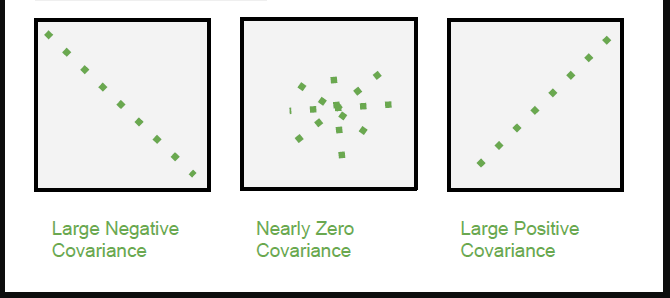
\includegraphics[trim={1cm 1cm 1cm 0}, clip, scale=0.4]{eda/cov.png}
		\caption{https://www.statisticshowto.com/covariance/}
	\end{figure}
	
\end{frame}
% Slide-n
\begin{frame}[t]{Covariance}
	$$
	cov(x,y) = \frac{\sum{(x_i - \overline{x})(y_i - \overline{y})}}{n-1}	
	$$
	\begin{itemize}
		\item $cov(x,y)$ $\rightarrow$ covariance between $x$ and $y$
		\item $x_i$ $ \rightarrow$ data value of $x$
		\item $y_i$ $\rightarrow$ data value of $y$
		\item $\overline{x}$ $\rightarrow$  mean of $x$
		\item $\overline{y}$ $\rightarrow$ mean of $y$
		\item $n$ $\rightarrow$ number of data values. 
	\end{itemize}
	
	
\end{frame}

% Slide-n
\begin{frame}[t]{Correlation}
	\begin{itemize}
		\item When two sets of data are strongly linked together we say they 
		have a High Correlation.
		\item Correlation is \textbf{Positive} when the values increase 
		together.
		\item Correlation is \textbf{Negative} when one value decreases as the 
		other increases
		\item A correlation is assumed to be linear.	
	\end{itemize}
	
	\begin{figure} [ht]
		\centering
		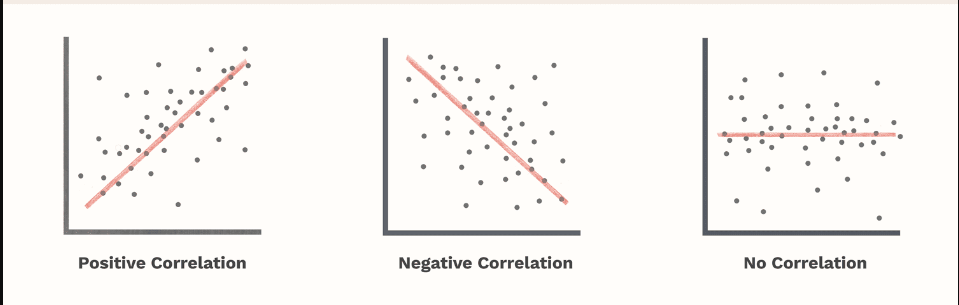
\includegraphics[trim={1cm 0cm 1cmcm 1cm}, clip, scale=0.4]{eda/corr}
	\end{figure}
\end{frame}

% Slide-n
\begin{frame}[t]{Interpretation}
	\begin{itemize}
		\item 1 is a perfect positive correlation
		\item 0 is no correlation (the values don't seem linked at all)
		\item -1 is a perfect negative correlation
	\end{itemize}
\end{frame}

% Slide-n
\begin{frame}[t]{Pearson's r Correlation}
	\begin{itemize}
		\item  Pearson's $r$ measures the strength of the linear relationship 
		between two variables.
		\item Pearson's $r$ is always between -1 and 1 
	\end{itemize}
	
	\begin{equation*}
	r =
	\frac{ \sum_{i=1}^{n}(x_i-\bar{x})(y_i-\bar{y}) }{%
		\sqrt{\sum_{i=1}^{n}(x_i-\bar{x})^2}\sqrt{\sum_{i=1}^{n}(y_i-\bar{y})^2}}
	\end{equation*}
	
	
	
	\begin{itemize}
		\item $r$ $\rightarrow$ correlation between $x$ and $y$
		\item $x_i$ $ \rightarrow$ data value of $x$
		\item $y_i$ $\rightarrow$ data value of $y$
		\item $\overline{x}$ $\rightarrow$  mean of $x$
		\item $\overline{y}$ $\rightarrow$ mean of $y$
	\end{itemize}
\end{frame}

% Slide-n
\begin{frame}[t]{Correlation Is Not Causation}
	\begin{itemize}
		\item A common saying is "Correlation Is Not Causation".
		\item What it really means is that a correlation does not prove one 
		thing causes the other.
		\item Causation means that one variable causes something to happen in 
		another variable.
		\item To say that two things are correlated is to say that they are not 
		some kind of relationship.
		\item In order to imply causation, a true experiment must be performed 
		where subjects are randomly assigned to different conditions.
	\end{itemize}
\end{frame}

% covariance & correlation 
% Slide-n
\begin{frame}[t]{Skewness}
	\textbf{Skewness:} 
	A measure of asymmetry around the mean.
	
	\begin{itemize}
		\item Normally distributed data: skewness = 0
		\item Extreme values are equally likely on both
		sides of the mean
		\item Symmetry about the mean
	\end{itemize}
\end{frame}


% Slide-n
\begin{frame}[t]{Positive Skewness}
	\begin{itemize}
		\item Consider incomes of individuals
		
		\item Billionaires: positive skew
		
		\item Outliers greater than mean more likely
		than outliers less than mean
		\item Right-skewed distribution
		\item Often seen when lower bound but no
		upper bound
		
	\end{itemize}
\end{frame}
% skewness

% Slide-n
\begin{frame}[t]{Kurtosis}
	\textbf{Kurtosis:} 
	Measure of how often extreme values (on either side of
	the mean) occur. \\ 
	Kurtosis is a statistical measure that defines how heavily the tails of a 
	distribution differ from the tails of a normal distribution. In other 
	words, 
	kurtosis identifies whether the tails of a given distribution contain 
	extreme 
	values.
	\begin{itemize}
		\item Normally distributed data: kurtosis = 3
		\item Excess kurtosis = kurtosis - 3
		\item Kurtosis Tail risk
		\item High kurtosis extreme events more
		likely than in normal distribution.
	\end{itemize}
\end{frame}

% Slide-n
\begin{frame}[t]{Distribution}
	\begin{figure}[h]
		\centering
		\begin{subfigure}{0.45\textwidth}
			\centering
			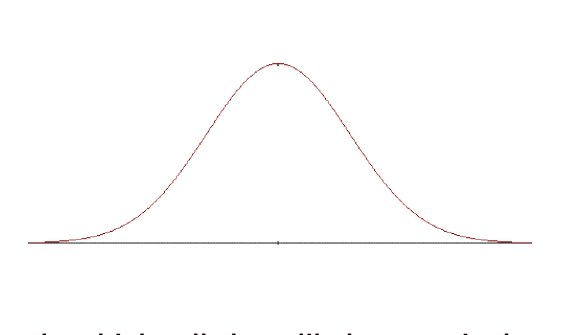
\includegraphics[trim={0 1cm 0 0}, clip, scale=0.4]{eda/nd.png}
			\caption{Values close to the mean are more likely}
		\end{subfigure}
		\hfil
		\begin{subfigure}{0.45\textwidth}
			\centering
			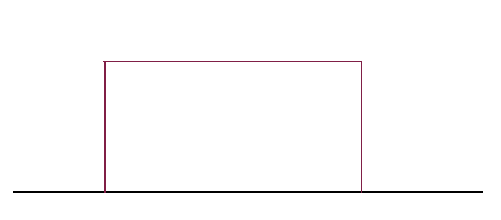
\includegraphics[scale=0.5]{eda/nd2.png}
			\caption{All values are equally likely}
		\end{subfigure}
		
	\end{figure}
\end{frame}

\begin{frame}[t]{The Normal Curve}
	\begin{itemize}
		\item The distributions of most continuous random variables will follow 
		the shape of the normal curve.
		\item Mean, Median and Mode all exist at the center.
		
	\end{itemize}
	\begin{figure} [ht]
		\centering
		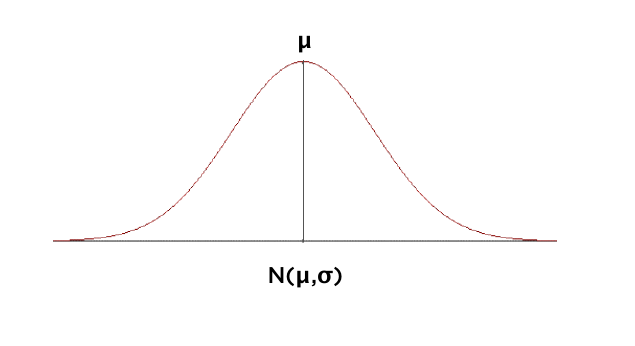
\includegraphics[trim={0 1cm 0 0}, clip, scale=0.4]{eda/nd3.png}
	\end{figure}
	\centering
	A formula which tells how likely a particular value is
	to occur in your data.
\end{frame}
% Slide-n
\begin{frame}[t]{The Empirical Rule--1}
	The empirical rule tells you what percentage of your data falls within a 
	certain number of standard deviations from the mean.
	\begin{itemize}
		\item 68\% of all values fall within 1 standard deviation of the mean.
		\item 95\% of the all values fall within 2 standard deviation of the 
		mean. 
		\item 99.7\% of the all values fall within 3 standard deviation of the 
		mean. 
	\end{itemize}
	
	\begin{figure} [ht]
		\centering
		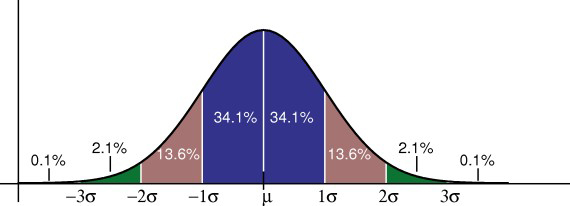
\includegraphics[width=0.5\textwidth]{eda/standard-normal-distribution.jpg}
		\caption{\url{https://www.statisticshowto.com/probability-and-statistics/normal-distributions/}}
	\end{figure}
\end{frame}


\begin{frame}[t]{The Empirical Rule--2}
	
	\begin{figure} [ht]
		\centering
		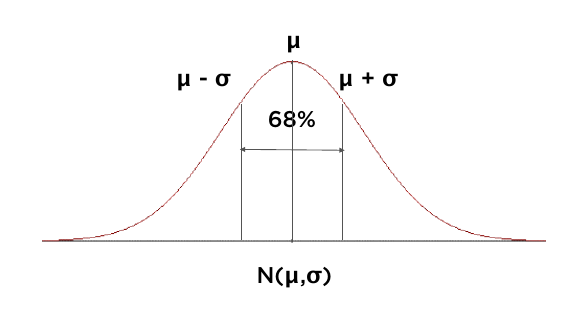
\includegraphics[trim={0 1cm 0 0}, clip, scale=0.4]{eda/nd7.png}
	\end{figure}
	
	\centering
	68\% within 1 standard deviation of mean
	
\end{frame}

\begin{frame}[t]{The Empirical Rule--3}
	
	\begin{figure} [ht]
		\centering
		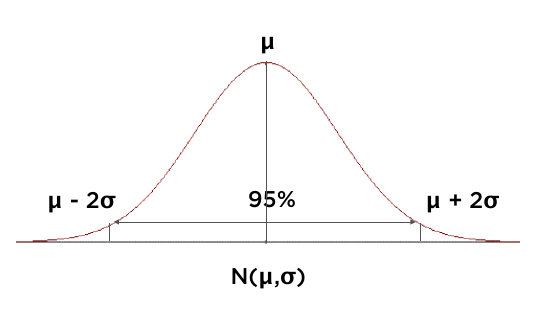
\includegraphics[trim={0 1cm 0 0}, clip, scale=0.4]{eda/nd8.png}
	\end{figure}
	
	\centering
	95\% within 2 standard deviations of mean
	
\end{frame}


\begin{frame}[t]{The Empirical Rule--4}
	
	\begin{figure} [ht]
		\centering
		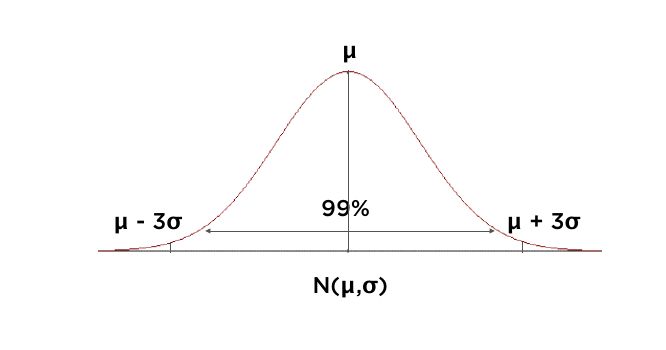
\includegraphics[trim={0 1cm 0 0}, clip, scale=0.4]{eda/nd9.png}
	\end{figure}
	
	\centering
	99\% within 3 standard deviations of mean
	
\end{frame}

\begin{frame}[t]{Impact of Outliers}
	
	\begin{figure} [ht]
		\centering
		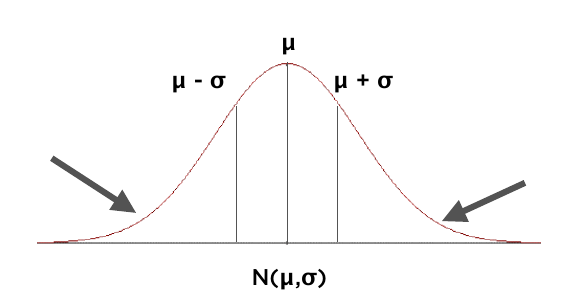
\includegraphics[trim={0 1cm 0 0}, clip, scale=0.4]{eda/nd6.png}
	\end{figure}
	
	\centering
	There will be few extreme values - the
	number of extreme values at either side of
	the mean will be the same.
\end{frame}

% Slide-n
\begin{frame}[t]{Properties of a Normal Distribution}
	\begin{itemize}
		\item The mean, mode and median are all equal.
		\item The curve is symmetric at the center (i.e. around the mean, 
		$\mu$).
		\item Exactly half of the values are to the left of center and exactly 
		half the values are to the right.
		\item The total area under the curve is 1.
	\end{itemize}
	
	\begin{figure} [ht]
		\centering
		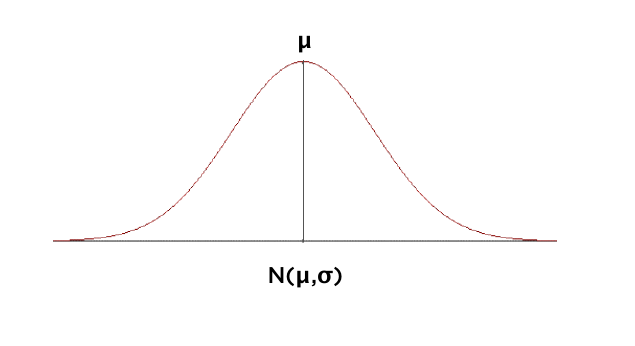
\includegraphics[trim={0 1cm 0 0}, clip, scale=0.4]{eda/nd3.png}
	\end{figure}
\end{frame}

% Slide-n
\begin{frame}[t]{Role of Sigma($\sigma$)}
	\begin{figure}[h]
		\centering
		\begin{subfigure}{0.45\textwidth}
			\centering
			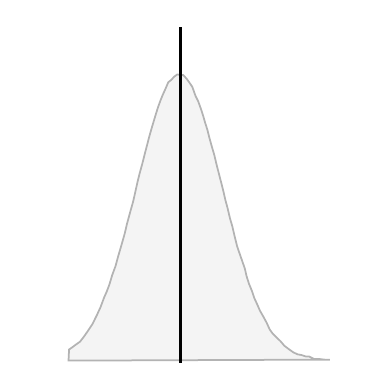
\includegraphics[scale=0.5]{eda/std1.png}
			\caption{Small Standard Deviation($\sigma$)}
			Few points far from the mean
		\end{subfigure}
		\hfil
		\begin{subfigure}{0.45\textwidth}
			\centering
			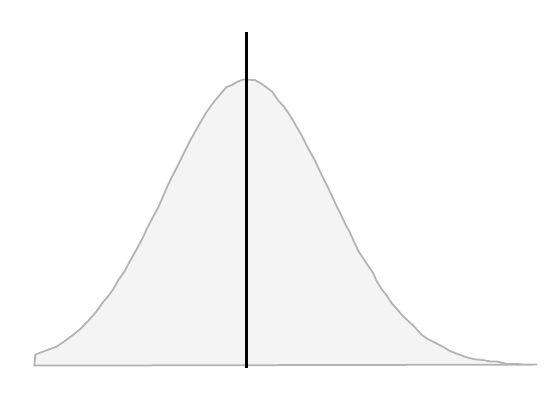
\includegraphics[scale=0.5]{eda/std2.png}
			\caption{ Large Standard Deviation($\sigma$)}
			Many points far from the mean
			
		\end{subfigure}
		
	\end{figure}
\end{frame}
% Slide-n
\begin{frame}[t]{Z-Scores}
	\begin{itemize}
		\item Z-Scores are standardized values that can be used to compare 
		scores in different distributions.
		\item Simply put, a z-score (also called a standard score) gives you an 
		idea of how far from the mean a data point is. But more technically 
		it’s a measure of how many standard deviations below or above the 
		population mean a raw score is.
		\item A z-score can be placed on a normal distribution curve. Z-scores 
		range from -3 standard deviations (which would fall to the far left of 
		the normal distribution curve) up to +3 standard deviations (which 
		would fall to the far right of the normal distribution curve). 
		\item In order 
		to use a z-score, you need to know the population mean $\mu$ and also 
		the 
		population standard deviation $\sigma$.
	\end{itemize}
	
\end{frame}

% Slide-n
\begin{frame}[t]{Calculating Z-Score}
	$$
	Z = \frac{\overline{x}-\mu}{\sigma}
	$$
	
	\begin{itemize}
		\item $\overline{x}$ $\rightarrow$ mean 
		\item $\mu$ $\rightarrow$ population mean 
		\item $\sigma$ $\rightarrow$ population standard deviation
	\end{itemize}
\end{frame}


% Slide-n
\begin{frame}[t]{Calculating Z-Score}
	For example, let’s say you have a test score of 190. The test has a mean 
	($\mu$) of 150 and a standard deviation ($\sigma$) of 25. Assuming a normal 
	distribution, your z score would be
	
\end{frame}


% Slide-n
\begin{frame}[t]{Skewness--1}
	\begin{itemize}
		\item A measure of asymmetry around the mean.
		\item If one tail is longer than another, the distribution is skewed.
		\item These distributions are sometimes called asymmetric or 
		asymmetrical distributions as they don’t show any kind of symmetry.
		\item Symmetry means that one half of the distribution is a mirror 
		image of the other half.
	\end{itemize}
	\begin{figure} [ht]
		\centering
		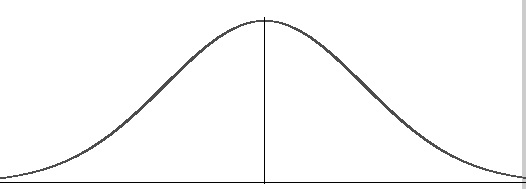
\includegraphics[trim={0 0 0.1cm 0}, clip, 
		scale=0.5]{eda/normal-distribution-probability.jpg}
		\caption{https://www.statisticshowto.com/probability-and-statistics/}
	\end{figure}
\end{frame}

\begin{frame}[t]{Skewness--2}
	\begin{itemize}
		\item Normally distributed data: skewness = 0
		\item Extreme values are equally likely on both
		sides of the mean.
		\item Symmetry about the mean
	\end{itemize}
	\begin{figure} [ht]
		\centering
		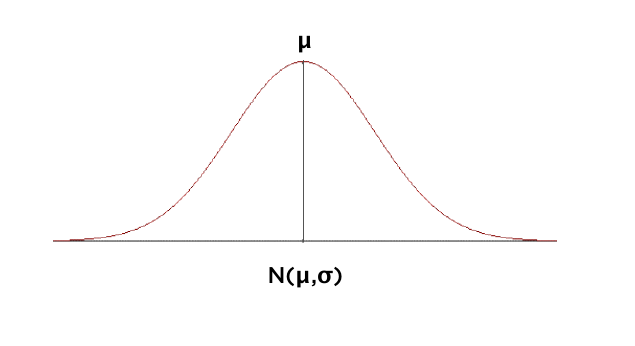
\includegraphics[trim={0 1cm 0 0}, clip, scale=0.4]{eda/nd3.png}
	\end{figure}
\end{frame}
% Slide-n
\begin{frame}[t]{Negative Skewness}
	\begin{itemize}
		\item A left-skewed distribution has a long left tail.
		\item Left-skewed distributions are also called negatively-skewed 
		distributions.
		\item That’s because there is a long tail in the negative direction on 
		the number line. The mean is also to the left of the peak.
	\end{itemize}
	
	\begin{figure} [ht]
		\centering
		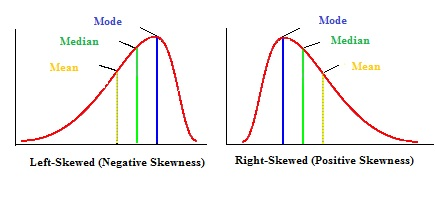
\includegraphics[trim={0 0 6cm 0}, clip, 
		scale=0.7]{eda/pearson-mode-skewness.jpg}
		\caption{\url{https://www.statisticshowto.com/probability-and-statistics/}}
	\end{figure}
\end{frame}

\begin{frame}[t]{Positive Skewness}
	\begin{itemize}
		\item A right-skewed distribution has a long right tail. 
		\item Right-skewed distributions are also called positive-skew 
		distributions.
		\item That’s because there is a long tail in the positive direction on 
		the number line. The mean is also to the right of the peak.
	\end{itemize}
	
	\begin{figure} [ht]
		\centering
		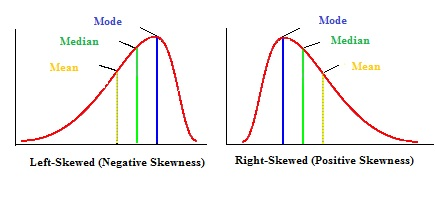
\includegraphics[trim={6cm 0 0 0}, clip, 
		scale=0.7]{eda/pearson-mode-skewness.jpg}
		\caption{\url{https://www.statisticshowto.com/probability-and-statistics/}}
	\end{figure}
\end{frame}


% Slide-n
\begin{frame}[t]{Mean and Median in Skewed Distributions}
	In a normal distribution, the mean and the median are the same 
	number while the mean and median in a skewed distribution become 
	different numbers.
	\begin{itemize}
		\item A left-skewed, negative distribution will have the mean to the 
		left of the median.
	\end{itemize}
	\begin{figure} [ht]
		\centering
		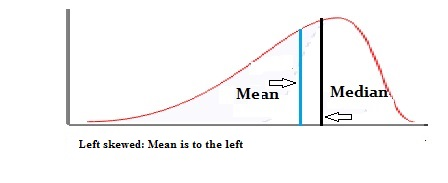
\includegraphics[width=0.6\textwidth]{eda/left-skewed.jpg}
		\caption{\url{https://www.statisticshowto.com/probability-and-statistics/}}
	\end{figure}
\end{frame}

% Slide-n
\begin{frame}[t]{Mean and Median in Skewed Distributions}
	\begin{itemize}
		\item A right-skewed, negative distribution will have the mean to the 
		right of the median.
	\end{itemize}
	\begin{figure} [ht]
		\centering
		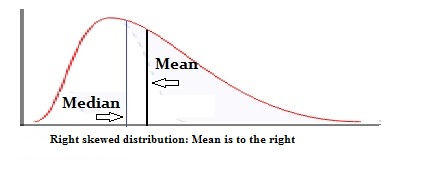
\includegraphics[width=0.6\textwidth]{eda/right-skewed.jpg}
		\caption{\url{https://www.statisticshowto.com/probability-and-statistics/}}
	\end{figure}
\end{frame}






\end{document}


